% !TEX root =  ../thesis.tex

\section{Introduction}
\label{sec:theory_introduction}

To carry the annotations from the source program to the target, a \emph{witness relation} is built for every transformation. The generated witness is also used to check the correctness of the transformation, since it can be verified independently from the transformation. This makes the witness a very convenient and powerful abstraction, because proving its correctness is simpler than proving the formal correctness of a transformation, that is generally very complex. In a modern compiler, for example, even the simplest transformation can be made up of thousands of line of code. Witnessing a transformation is a new idea in the field of formal methods and compilers, and as such, it needs a formal definition that can be used in the theorems and hypotheses about its properties. From a theoretical point of view, the layout of witness generation is simple, yet, defining and proving its completeness requires some non-trivial demonstrations. In this chapter the concept of \emph{stuttering simulation} is also introduced, and it is shown that establishing a stuttering simulation relation from target to source is a sound and complete method for proving correctness.

The theory that is being presented inside this chapter was developed by Zuck and Namjoshi, in the paper called ``Witnessing Program Transformations''\cite{zucknamjoshi}. A briefer approach is given in \cite{namjzucktag}, where the results of this work are summarized.
% In this paper the theory behind the approach of witnessing the transformation is developed for the first time. The definitions that described the mathematical concepts are introduced, the theorems regarding the witness are expressed and a demonstration is laid out for almost all of them. This work draws from that paper the theory that is needed to build the framework implementation. Trying to define a new theory is far from the scope of this work, that instead aims at designing a framework and implementing it, based on the theory presented in this chapter. In some cases, however, the format of the mathematical object is modified in order to be consistent to the implementation, where the theory is manipulated in different ways for different reason (implementation, optimality, easiness of use). Clearly the new reformulation doesn't jeopardize the theoretical conclusions obtained with the original definition presented in the paper. Where it's possible the theorem formulation is taken as the same, in order not to lose formal correctness, and the demonstrations are not presented. For the formal demonstrations one can refer to the paper previously mentioned.

% In Chapter~\ref{cha:witness_for_common_optimizations} the idea of witness is applied to some common optimizations, to illustrate some features of witness generation. Subsequently, In Chapter~\ref{cha:hacking_llvm} the same problem is approached from the implementation side: a witness generator implementation is designed, and some witness-enhanced transformations are built for the LLVM Compiler, and which problems and difficulties have to be considered in order to build a correct implementation.

\section{Definitions}
\label{sec:definition}

The definitions presented in this section are basically the one used in \cite{zucknamjoshi}, with some minor changes to fit the implementation.

% In order to write the formal definition of witness, first some preliminary concepts need to be defined, which will be used later on to demonstrate useful properties of the witness relation. These definitions follow an incremental approach, That will end with the demonstration of these concepts in relation to some concrete transformation passes.

\begin{fdefinition}[Program]
\label{def:program}
A program is described as a tuple $(V, G, T, I)$, where
\begin{itemize}
  \item $V$ is a finite set of (typed) variables
  \item $G$ is a finite directed graph (it can be, for example, the control-flow graph)
  \item $T$ is a function specifying, for every edge $(i, j) \in G$, a symbolic transition condition denoted $T_{i,j}(V, V')$. Primed variables are used to denote the value of the program variables at the program state after the transition
  \item $I(V)$ is an initial condition for the program
\end{itemize}
\end{fdefinition}

\begin{figure}[ht]
  \begin{mdframed}
  \vspace{1cm}
  \centering
  \begin{tikzpicture}[%
    ->,
    shorten >=2pt,
    >=stealth,
    node distance=1cm,
    noname/.style={%
      ellipse,
      minimum width=5em,
      minimum height=3em,
      draw}
    ]
  \node[noname] (1) {\textbf{S}};
  \node[noname] (2) [below=of 1] {2};
  \node[noname] (4) [node distance=1cm and 3mm,below left=of 2] {4};
  \node[noname] (3) [left=of 4] {3};
  \node[noname] (5) [below=of 4] {5};
  \node[noname] (6) [node distance=2cm,right=of 5] {\textbf{F}};
  \path (1) edge node{} (2)
        (2) edge node{} (3)
        (2) edge node{} (4)
        (2) edge node{} (6)
        (3) edge node{} (5)
        (4) edge node{} (5)
        (5) edge [bend right=20pt] node {} (2);
  \node [bordered] at (2,0) {\texttt{x=1}\\\texttt{y=1}};
  \node [bordered] at (4,-6) {\texttt{x=0}\\\texttt{y=2}};
  \draw  (-1,1) rectangle (3,-1);
  \draw  (1,-5) rectangle (5,-7);
  \node [] at (2,0.6) {s};
  \node [] at (4,-5.4) {f};
  \node [] at (-0.1,1.2) {State $(\textbf{S},s)$};
  \node [] at (1.9,-4.8) {State $(\textbf{F},f)$};
  \end{tikzpicture}
  \vspace{1cm}
  \end{mdframed}
  \caption[Example of graph $G$]{Example of graph $G$. A pair $(l,v)$ is a \emph{state}. State $(\textbf{S},s)$ is \emph{initial}, State $(\textbf{F},f)$ is \emph{final}}
  \label{fig:programcfg}
\end{figure}

Every transition relates current and next-state values of the variables. $G$ has two distinguished nodes, $\textbf{S}$ and $\textbf{F}$. The $\textbf{S}$ node has no incoming edges, and the $\textbf{F}$ node has no outgoing edges, meaning that from $F$ no transition can be triggered (see Figure~\ref{fig:programcfg}). In this work we assume that every program P is deadlock-free, meaning that only the node $\textbf{F}$ has no enabled outgoing transition.
% A further assumption is that the program is not guaranteed to terminate, i.e., it can reach  $\textbf{F}$ from any node. In this case the program computation starves.

A \emph{state} of a program is given by a pair $(l, v),$ where $l$ is a node of $G$ and $v$ is type-consistent assignment of values to each variable in $V$. A state is defined as \emph{initial} if and only if $ l = \textbf{S} \land I(v)$ holds.
% A state such that $ l = \textbf{S} \land !I(v)$ is an invalid initial state for the program.
A state is \emph{final} if and only if $ l = \textbf{F}$.

A transition system can be defined w.r.t. the program definition as follows.

\begin{fdefinition}[Transition System]
A transition system $T$ is given by a tuple $(S,I,R)$ where:

\begin{itemize}
  \item $S$ is a set of states,
  \item $I$ is the subset of initial states (i.e. inputs),
  \item $R \subseteq S \times S$ is a transition relation
\end{itemize}
\end{fdefinition}

A program $P(V, G, T, I)$ (as definied in Definition~\ref{def:program}) induces the transition system where the states are interpretations of $V$, the initial states are the those in $I$, and the relation $R$ is that defined symbolically by $T$. Using the definition of transition system instead of the program in the simulation definition will simplify them, without losing generality.

Moreover, a \emph{program computation} of lenght $n$ is a sequence of states $s_0, s_1 ,\ldots s_n$ where $s_0$ is initial and for each pair $s_i=(l_i,v_i), s_{i+1}=(l_{i+1},v_{i+1})$ of consecutive states on the sequence, $(l_i, l_i+1)$ is an edge in $G$, and the transition condition $T_{i,i+1}(v_i,v_i+1)$ holds.

A computation can have infinite length. A computation is \emph{terminating} if $s_n = (\textbf{F},v_n)$. A computation is \emph{maximal} when no transition can be enabled from the last state, i.e., when it's terminating or infinite.

\begin{fdefinition}[State Matching]
Let $T$, $S$ be two programs and $T_T(S_T,I_T,R_T)$,$T_S(S_S,I_S,R_S)$ the corresponding transition relations. States $t \in S_T$ and $s \in S_S$ match, denoted $t \simeq s$, if $t$ and $s$ assign the same value to every variable $v \in V' = V_S \cap V_T$.
\end{fdefinition}

\begin{fdefinition}[Path Matching]
\label{def:path_matching}
For Programs $T$ and $S$ a maximal computation $\tau$ of program $T$ is \emph{matched} by a maximal computation of $\sigma$ of program $S$ if the following conditions all hold:
\begin{itemize}
  \item The starting state of $T$ and $S$ match
  \item if $(\textbf{F}_T,v) \in \tau$ for some variable assignment $v$, then for some $w$, $(\textbf{F}_S,w) \in \sigma$
  \item if $\sigma$ has no final state, neither does $\tau$
\end{itemize}

% The second and third conditions can be equivalently substituted by the following condition: $(\textbf{F}_T,v) \in \tau \iff (\textbf{F}_S,w) \in \sigma$.

\end{fdefinition}

\begin{fdefinition}[Implementation]
Given two programs, $T$ and $S$, $T$ \emph{implements} $S$ if for every maximal computation $\tau$ of $T$, there is a maximal computation $\sigma$ of $S$ that matches it.
\end{fdefinition}

If $T$ implements $S$, then every terminating computation of $T$ has a corresponding terminating computation of $S$ starting from a matching initial state such that the final states (if any) also match. Hence, the input-output relation of $T$ is included in that of $S$, w.r.t. the common variables. Moreover, if $T$ has a non-terminating computation from some initial state, non-termination is also possible for $S$ from a matching state. This disallows, for example, pathological ``implementations'' where $T$ has no terminating computations, so that the input-output relation of $T$ (the empty set) is trivially contained in the input-output relation of $S$.

\begin{fdefinition}[Transformation Function]
A \emph{transformation} is a \emph{partial} function on the set of programs. A transformation $\delta$ is \emph{correct} if for every program $S$ in its domain, $T=\delta (S)$ implements $S$.
\end{fdefinition}

In practical terms, a transformation is partial because it needs not to apply to all programs. Indeed, much of the effort in compiler optimization is on the analysis required to determine whether a particular transformation can be applied. This is a very important point, that enforces the idea that, from a theoretical point of view, verifying the witness is much easier than verifying the whole transformation. It should be remembered also that the witnessing approach doesn't try to verify the correctness of the transformation over all legal inputs. As translation validation approach \cite{pnueli1998translation}, the witness aims at verifying that an instance of transformation produced an output that implements the input.

\section{Simulation relations}
\label{sec:stuttering_simulation}

Now we introduce two different kind of transition relations: Step and Stuttering Simulation. Both of them can be used as witness format, since, as it will be pointed out below, both can guarantee that the target program is a correct implementation of the source. The basic difference between the two relations is in terms of the kind of transformation that can be witnessed. A proof of the properties of the simulation is sketched but not formally expressed. The complete demonstrations are laid out in \cite{zucknamjoshi}.

\begin{fdefinition}[Step Simulation]
Given the transition systems $T$ and $S$, a relation $X \subseteq S_T \times S_S$ is a \emph{step simulation} if:
\begin{itemize}
  \item the domain of $X$ includes all initial states of $T$
  \item for any $(t,s) \in X$, $t$ and $s$ satisfy the same propositions and for every $t'$ such that $t,t' \in R_T$, there is a $s'$ such that $(s,s') \in R_S$ and $(t',s') \in X$.
\end{itemize}
\end{fdefinition}

It is shown in \cite{zucknamjoshi} that step simulation guarantees that the target program is a correct implementation of the source:

\begin{ftheorem}[Step Soundness\cite{zucknamjoshi}]
\label{thm:step_soundness}
  For programs $T$ and $S$, $T$ implements $S$ if there is a step simulation $X(S_S\times S_T)$ from the states of every $T$-computation to the states of $S$-computation such that:
  \begin{itemize}
    \item for every initial state $s_{T}$ of $T$ there is an initial state $s_{S}$ such that $(s_{T},s_{S}) \in X$
    \item for every final state $t_{T}$ of $T$, if  $(t_{T},t_{S}) \in X$ then $t_{S}$ is a final state of $S$
  \end{itemize}
\end{ftheorem}
Thus, checking the single-transition conditions of step simulation, together with the two additional conditions of Theorem~\ref{thm:step_soundness}, is enough to show that $T$ implements $S$. These checks can be encoded as correctness questions and resolved with an automatic decision procedure.

However, it is not always possible to draw a transition relation between a correctly implemented target and its source program. In fact, if a step simulation relation can be defined, for every step taken in the target transition, there is a corresponding step in the source transition. This obviously requires the two transitions to have the same exact length.

Stuttering Simulation Relation, the next witness format that is described, relaxes this exact, 1-1 matching by permitting $\tau$ and $\sigma$ to be matched in segments, as illustrated in Figure~\ref{fig:stuttering1}.

\begin{figure}[hb]
  \begin{mdframed}
  \vspace{1cm}
  \centering
  \begin{tikzpicture}
  \node [gcircle] (v) at (-2.5,1.5) {};
  \node [gcircle] (v1) at (-1.5,1.5) {};
  \node [gcircle] (v2) at (-0.5,1.5) {};
  \node [gcircle] (v3) at (0.5,1.5) {};
  \node [gcircle] (v4) at (1.5,1.5) {};
  \node [gcircle] (v5) at (2.5,1.5) {};
  \node [gcircle] (v6) at (3.5,1.5) {};
  \node [gcircle] (v7) at (4.5,1.5) {};
  \node [gcircle] (v8) at (-2.5,0) {};
  \node [gcircle] (v9) at (-1.5,0) {};
  \node [gcircle] (v10) at (-0.5,0) {};
  \node [gcircle] (v11) at (0.5,0) {};
  \node [gcircle] (v12) at (1.5,0) {};
  \node [gcircle] (v13) at (2.5,0) {};
  \node [gcircle] (v14) at (3.5,0) {};
  \node [gcircle] (v15) at (4.5,0) {};
  \draw [densely dashed] (v8) edge (v);
  \draw [densely dashed] (v) edge (v9);
  \draw [densely dashed] (v10) edge (v);
  \draw [densely dashed] (v1) edge (v11);
  \draw [densely dashed] (v2) edge (v12);
  \draw [densely dashed] (v12) edge (v3);
  \draw [densely dashed] (v4) edge (v12);
  \draw [densely dashed] (v5) edge (v14);
  \draw [densely dashed] (v13) edge (v5);
  \draw [densely dashed] (v15) edge (v7);
  \draw [densely dashed] (v6) edge (v15);
  \draw [arrow] (v) edge (v1);
  \draw [arrow] (v1) edge (v2);
  \draw [arrow] (v2) edge (v3);
  \draw [arrow] (v3) edge (v4);
  \draw [arrow] (v4) edge (v5);
  \draw [arrow] (v5) edge (v6);
  \draw [arrow] (v6) edge (v7);
  \draw [arrow] (v8) edge (v9);
  \draw [arrow] (v9) edge (v10);
  \draw [arrow] (v10) edge (v11);
  \draw [arrow] (v11) edge (v12);
  \draw [arrow] (v13) edge (v14);
  \draw [arrow] (v12) edge (v13);
  \draw [arrow] (v14) edge (v15);
  \draw  (-3,2) rectangle (5,1);
  \node [] at (-3.2,1.9) {\huge{$\tau$}};
  \draw  (-3,0.5) rectangle (5,-0.5);
  \node [] at (-3.2,0.35) {\huge{$\sigma$}};
  \end{tikzpicture}
  \vspace{1cm}
  \end{mdframed}
  \caption{Stuttering Simulation}
  \label{fig:stuttering1}
\end{figure}

It has been demonstrated\cite{namjoshi1997simple} that the segments can be replaced by single steps, adding an additional dimension to the stuttering simulation relation. This is done by adding a \emph{ranking function} $Rank: (T,S) \rightarrow \mathbb{N}$ which decreases strictly at each stuttering step. In this work a simpler form of stuttering simulation is necessary.

\begin{figure}[ht]
  \begin{mdframed}
  \vspace{1cm}
  \centering
  \begin{subfigure}[b]{0.3\textwidth}
    \centering
    \begin{tikzpicture}
    \node [gcircle, minimum size = 23] (u) at (-2.5,2) {$t$};
    \node [gcircle, minimum size = 23] (u1) at (0,2) {$t'$};
    \node [gcircle, minimum size = 23] (v) at (-2.5,0) {$s$};
    \node [gcircle, minimum size = 23] (v1) at (0,0) {$s'$};

    \draw [densely dashed, arrow] (u) edge node[midway,auto] {$X$} (v);
    \draw [densely dashed, arrow] (u1) edge node[midway,auto] {$X$} (v1);

    \draw [arrow] (v) edge (v1);
    \draw [arrow] (u) edge (u1);
    \end{tikzpicture}
    \caption{Case 1}
    \label{fig:stuttering21}
  \end{subfigure}
    \begin{subfigure}[b]{0.3\textwidth}
    \centering
    \begin{tikzpicture}
    \node [gcircle, minimum size = 23] (u) at (-2.5,2) {$t$};
    \node [gcircle, minimum size = 23] (u1) at (0,2) {$t'$};
    \node [gcircle, minimum size = 23] (v) at (-2.5,0) {$s$};
    \node [gcircle, minimum size = 23] (v1) at (0,0) {$s'$};

    \draw [densely dashed, arrow] (u) edge node[midway,auto] {$X$} (v);
    \draw [densely dashed, arrow] (u) edge node[midway,auto] {$X$} (v1);

    \draw [arrow] (v) edge node[midway,auto] {$V$} (v1);
    \draw [arrow] (u) edge (u1);
    \node at (-1.8,1) {\Large{$\prec$}};
    \end{tikzpicture}
    \caption{Case 2}
    \label{fig:stuttering22}
  \end{subfigure}
    \begin{subfigure}[b]{0.3\textwidth}
    \centering
    \begin{tikzpicture}
    \node [gcircle, minimum size = 23] (u) at (-2.5,2) {$t$};
    \node [gcircle, minimum size = 23] (u1) at (0,2) {$t'$};
    \node [gcircle, minimum size = 23] (v) at (-2.5,0) {$s$};

    \draw [densely dashed, arrow] (u) edge node[midway,auto] {$X$} (v);
    \draw [densely dashed, arrow] (u1) edge node[midway,auto] {$X$} (v);

    \draw [arrow] (u) edge (u1);
    \node at (-1.8,1) {\Large{$\prec$}};
    \end{tikzpicture}
    \caption{Case 3}
    \label{fig:stuttering23}
  \end{subfigure}
  \vspace{1cm}
  \end{mdframed}
  \caption{Stuttering Simulation with ranking}
  \label{fig:stuttering2}
\end{figure}

\begin{fdefinition}[Stuttering Simulation with Ranking function]
\label{def:stuttering_simulation}
Given Transition systems $B$ and $A$, a relation $ X \subseteq S_T \times S_S $ augmented with a partial ranking function, $Rank: (S_T,S_S) \rightarrow \mathbb{N}$, over a well-founded domain $(\mathbb{N},\prec)$, is a \emph{stuttering simulation} if:
\begin{itemize}
  \item the domain of $X$ includes all initial states of $T$ and
  \item for any $(t, s) \in X$, $t$ and $s$ satisfy the same propositions and for every $t'$ such that $(t,t') \in R_T$, one of the following holds:
  \begin{itemize}
    \item There is $s'$ such that $(s,s') \in R_S \land (t',s') \in X$ (Figure~\ref{fig:stuttering21}), or
    \item There is $s'$ such that $(s,s') \in R_S \land (t,s') \in X \land rank(t,s') \prec rank(t,s)$ (stuttering on A, Figure~\ref{fig:stuttering22}), or
    \item $(t',s) \in X$ and rank $(t',s) \prec (t,s)$ (stuttering on B, Figure~\ref{fig:stuttering23}).
  \end{itemize}
\end{itemize}
\end{fdefinition}

A graphical explanation of this definition is given in Figure~\ref{fig:stuttering2}. It is immediate to observe how step simulation is a specialization of stuttering simulation. If we define three sets $\mathcal{REL},\mathcal{STUT},\mathcal{STEP}$ as the set of all general relations, step simulation relations and stuttering simulation relations respectively, we have $\mathcal{STEP} \subset \mathcal{STUT} \subset \mathcal{REL}$ (Figure~\ref{fig:relations}). This result will help to clarify some considerations. While $\mathcal{REL}$ can define every transformation relation from program $A$ to $B$, not all are correct (i.e, $B=X(A)$ implements $A$). On the other hand, this is true for all the step simulations (Theorem~\ref{thm:step_soundness}), yet, as already stated before, step simulation is too restrictive in terms of transformations that can be simulated. In fact, it can be applied only when the the transformation doesn't rearrange, eliminate or add instructions. Therefore, stuttering simulation is the best candidate to accommodate all kind of transformations, as it is, we'll observe, a sound and complete simulation. It must be considered also that the definition of stuttering simulation adds an additional dimension to the relation, that is the one defined by the ranking function that accompanies the stuttering simulation to guarantee that the lengths of the matched segment are finite. The figure doesn't take into account the ranking function, so it is a simplification of the actual property of stuttering simulation. In fact, as it is shown in \cite{zucknamjoshi}, without the ranking function it wouldn't be possible to demonstrate the completeness of the stuttering simulation.

\begin{figure}[ht]
  \begin{mdframed}
    \vspace{1cm}
    \centering
    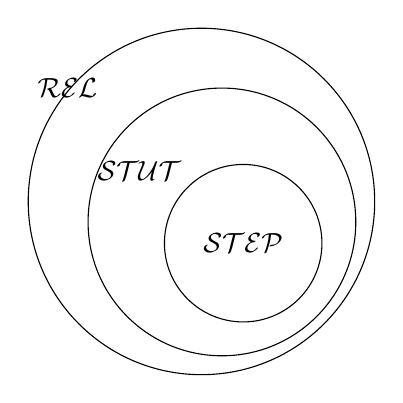
\begin{tikzpicture}
      \def\firstcircle{(0:0) circle (2.2cm)}
      \def\secondcircle{(0.26,-0.26cm) circle (1.7cm)}
      \def\thirdcircle{(0.53,-0.53cm) circle (1cm)}
      \draw \firstcircle node[above left = 1.2cm] {$\mathcal{REL}$};
        \draw \secondcircle node [above left = .4cm] {$\mathcal{STUT}$};
        \draw \thirdcircle node [] {$\mathcal{STEP}$};
    \end{tikzpicture}
    \vspace{1cm}
  \end{mdframed}
  \caption{Relation hierarchy}
  \label{fig:relations}
\end{figure}

\begin{ftheorem}[Soundness\cite{zucknamjoshi}]
\label{thm:soundness}
Let $X$ be a stuttering simulation relating states of a program $T$ to those of program $S$. Then $T$ is a correct implementation of $S$ when the following conditions all hold:
\begin{itemize}
  \item For every initial state $s$ of $S$, there is an initial state $t$ of $T$ such that $(t, s) \in X $ and $ t \simeq s$.
  \item Final states of $S$ or $T$ are $X$-related to only final states of the other program. Moreover, if $t$ and $s$ are $X$-related final states of $T$ and $S$, then $t \simeq s$.
\end{itemize}
\end{ftheorem}

The conditions expressed in the soundness theorem gives the definition of \emph{Witness Relation}:

\begin{fdefinition}[Witness]
Let $S$ and $T$ be programs related by a stuttering simulation relation $W$ from the state space of $T$ to that of $S$. $W$ is a \emph{Witness relation} if the soundness conditions hold:
\begin{itemize}
  \item For every initial state $u$ of $T$, there is an initial state $v$ of $S$ such that $(u,v) \in W $ and $ u \simeq v$.
  \item Final states of $S$ or $T$ are $W$-related to only final states of the other program. Moreover, if $u$ and $v$ are $W$-related final states of $T$ and $S$, then $u \simeq v$.
\end{itemize}
In other words, that means that the stuttering simulation is a sound witness.
\end{fdefinition}

Based on Manolios\cite{manolios2003compositional}, Namjoshi and Zuck proved that stuttering simulation is sound and complete.
 % when augmented with history and prophecy variables, where prophecy variables are used only to overcome non-determinism. A specialization of Manolios' result is shown for programs where transitions are deterministic and the only non-determinism is the choice of initial state. In this specialization prophecy variables are unnecessary; moreover, w.r.t. to this work the history can be assumed by the definition of stuttering simulation. In practice, this is not a limitation, because internal representation of the compilers are statically deterministic.

% The following theorem has a very important result, because it shows that is always possible, at least in theory, to generate a witness, whatever transformation has occurred and whatever was the source program. The guarantee of completeness is a result that Translation Validation techniques lacks, as TV is applicable only to a certain set of transformation, and the proof is not guaranteed to be always found (\cite{zuck2005translation}).

% \begin{ftheorem}[Completeness]
% \label{thm:completeness}
% Consider programs $B$ and $A$ both of which have a deterministic transition relation. If $B$ refines $A$, there is a stuttering simulation relation between the programs augmented with history variables which meets the conditions of Theorem~\ref{thm:soundness}(Soundness Theorem).
% \end{ftheorem}

\section{Invariant propagation}
\label{sec:invariant_propagation}

A relation that satisfies the Witness format can also be used to ``propagate'' the assertions from end to end of the transformation pass, making the additional transformation to be used also in different part of the transformation process, rather than just by the first one. This result of this property is what the second problem pointed out in the introductory section. \emph{Propagation} informally means that if an assertion $\theta$ is true for a subset of source states $S_S' \in S_S$, the propagated assertion $\theta'$ must be true for all and only the target states $S_T' \in S_T$ where every state $t \in S_T'$ is related to some state $s \in S_S'$ by the witness relation $W$. Now a more formal description will be provided.

First we define the concept of pre-image of $\theta$ under $W$, denoted ($\langle W \rangle \theta$), as the set $\left\{(m,t) | (\in l,s : ((m,t),(l,s)) \in W \land \theta(l,s)\right\}$. The following theorem holds:

\begin{ftheorem}[Invariant Propagation\cite{zucknamjoshi}]
\label{thm:propagation}
Let $W$ be a stuttering simulation witness for a transformation from program $T$ to program $S$. If $\theta$ is an invariant for $S$, the set $\langle W \rangle \theta$ is an invariant for $T$. Moreover, if $\theta$ is inductive, so is $\langle W \rangle \theta$.
\end{ftheorem}
The sketch of the proof for the correctness of  $\langle W \rangle \theta$ as invariant at Target is as follows. Let $\theta$ be an invariant holding for every state of a program $S$. For every valid computation $\tau$ of program $T$, there must exist, from the definition of witness relation, a computation $\sigma$ of program $S$ such that $\forall t \in \tau, \exists s \in \sigma, W(t, s)$. It is true also that $\forall s \in \sigma, s \in \theta$. The last formula holds because $\sigma$ is a computation of S (where $\theta$ holds). Combining the last two formulas ensues that $\underset{t \in \tau}{\bigcup} \in \langle W \rangle \theta$. Hence, $\langle W \rangle \theta$ is a correct invariant for program $T$.

\section{Generalization}
\label{sec:generalization}
The transition relation can be generalized and adjusted to the concept of control-flow graph (CFG) of a program $P$. In this generalization, the states of a program refers only to the beginning of a basic block of the graph, and the transition relation maps every node of the CFG of the program to its successors. Hence, every transition can cover more than one instruction. The generalization is useful for two different reasons. This restricts the cases where step simulation is not sufficient and stuttering simulation is necessary,
% making the generation of the witness easier for these cases.

Consider the example of Dead Code Elimination. As it will be shown in the following chapter, DCE transformation can be witnessed by a stuttering simulation relation. However, if we generalize the transition relation to work over the basic blocks rather than single instructions, step simulation is sufficient to prove the correctness of this transformation. This is due to the fact that Dead code elimination doesn't change the CFG structure. Hence, it follows that stuttering simulation is usually necessary when the transformation reorders, eliminates, or add nodes of the Control Flow Graph.

The second reason is that many compilers, such as LLVM, build the CFG of the function as a preliminary step before every optimization pass. This implies that building the generalized relations over the existing CFG is a more efficient approach than building instruction-wise transitions.
